\section{Untapped enormous potential: integrating mobile devices into the Grid}
Now, with general understanding of what Grid Computing is and how mobile devices evolved over the years, the main topic of this work can be discussed: integrating (using volunteer computing) mobile devices into Grid Computing alongside desktop computers exploiting an enormous quantity of computational resources that lay unused in the pockets of billions of users.

\subsection{Idea: strength in numbers}
As seen in \textit{figure \ref{fig:global_sales_of_pcs_and_smartphones}}, the market has an enormous number of smartphones sold, thus resulting in an abundance of available devices that billions of users use every day (tablets have also to be taken in consideration).
\vspace{10mm}

\begin{figure}[!ht]
    \centering
    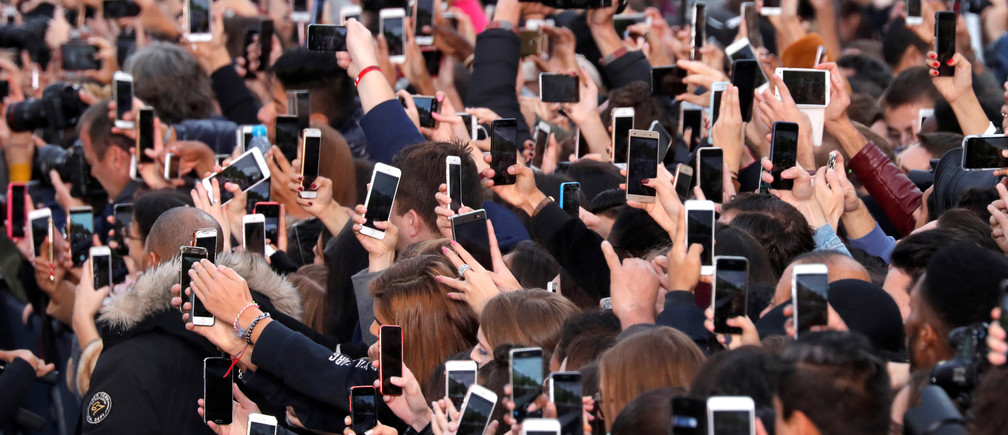
\includegraphics[scale=1.2]{document/chapters/chapter_1/images/people_using_smartphones.jpg}
    \caption{Smartphones are now used daily on a regular basis}
    \label{fig:people_using_smartphones}
\end{figure}

Despite smartphones and tablets are not on the same level (in terms of hardware capabilities) with current computers, it is possible to exploit the availability of a vast number of devices as a leverage to compensate the performances of such mobile devices.
This concept becomes increasingly relevant also considering the tendency of users to progressively use less and less desktop computers in favor of their mobile devices.

\subsection{Previous works and how limitations evolved}
A number of previous works discussed the idea and all of them agreed on the potential of exploiting mobile devices resources; quoting directly from the 2003 article \textit{"Should one incorporate Mobile-ware in Parallel and Distributed Computation?"} by Mustafa Sanver, Sathya Prya Durairaju and Ajay Gupta \cite{should_one_incorporate_mobile_ware}:
\begin{quotation}
    \textit{"At first glance, an individual mobile device may not have sufficient capacity and computational power for the integration. However, if we can harness the aggregated mobile power instead of individual power and consider exponential-rise of mobile units marketed and significantly evolving mobile technology, then one may conclude that it is worth the effort using this vast, pervasive, and untouched computational source for parallel computation."}
\end{quotation}

While recognizing the potential behind this concept, previous works pointed out to two important arguments against integrating mobile devices into Grid Computing:
\begin{itemize}
    \item Challenges inherently linked with adding mobile devices to the Grid, that this work will discuss in detail later in \textit{section TODO};
    \item Technical limitations, that will now be discussed in order to show how (mostly) they no longer apply, and thus this idea can be realized.
\end{itemize}

\subsubsection{Mobile devices competitive performances}
The first limitation that was pointed at was the poor performances of mobile devices; while this was certainly true for PDAs, as discussed in \textit{section \ref{technological_progress}}, today's smartphones and tablets do offer resources that are vastly more powerful than what was available in the past.

Wireless connectivity is also much stabler, faster and wildly available, especially considering the possibility of limiting participation to the Grid only while the device is connected to a Wi-Fi network.

The mobility factor of such devices is also not a limiting factors since one could argue that a volunteer that moves its device in space (thus possibly interrupting the connection to the Wi-Fi network) can be assimilated to a desktop volunteer that turns off its computer or is suddenly isolated from the network, reducing the mobility to a challenge inherently tied to Grid Computing.

\subsubsection{Mobile users common behavior}
TODO

\subsubsection{Economically sustainable internet connections}
TODO

\subsubsection{Standardized mobile market}
TODO

\subsubsection{Not only mobile: devices transparency principle}
TODO
